\subsection{Ondas estacionarias de som no tubo de Rubens}

Nesse último experimento utilizaremos um Tubo de Rubens e faremos uma série de medições a fim de conseguir a velocidade do som no gás ali presente.

Um Tubo de Rubens consiste em um cilindro metálico com perfurações equidistantes em sua parte superior e seus extremos fechados. Uma das extremidades é alimentada com um gás inflamável e, na outra, é instalado um gerador de frequência (alto falante).
Alimentamos o tubo com o gás e incendiamos o gás que escapa pelos furos superiores. 

Quando o alto-falante é ligado, a onda estacionária irá criar pontos com oscilação de pressão (anti-nós de pressão) e pontos com pressão constante (nós de pressão) ao longo do tubo. Quando há uma pressão devido às ondas sonoras, menos gás irá escapar das perfurações no tubo, e as chamas terão uma altura menor nesses pontos (fluxo de gás menor saindo pelo buraco). Nos nós de pressão, as chamas são mais elevados (fluxo de gás maior saindo pelo buraco). No final do tubo de gás, a velocidade das moléculas é zero e a pressão oscilante é máxima , assim são observados chamas baixas.
\begin{figure}[H]
  \centering
  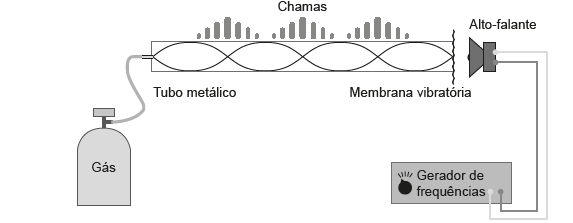
\includegraphics[scale=0.7]{images/Rub.png}
  \caption{Esquema do Tubo de Rubens}
\end{figure}    

O efeito das chamas, que variam de tamanho de acordo com a pressão, é algo visualmente bonito e que nos ensina muito sobre as ondas.

\begin{figure}[H]
  \centering
  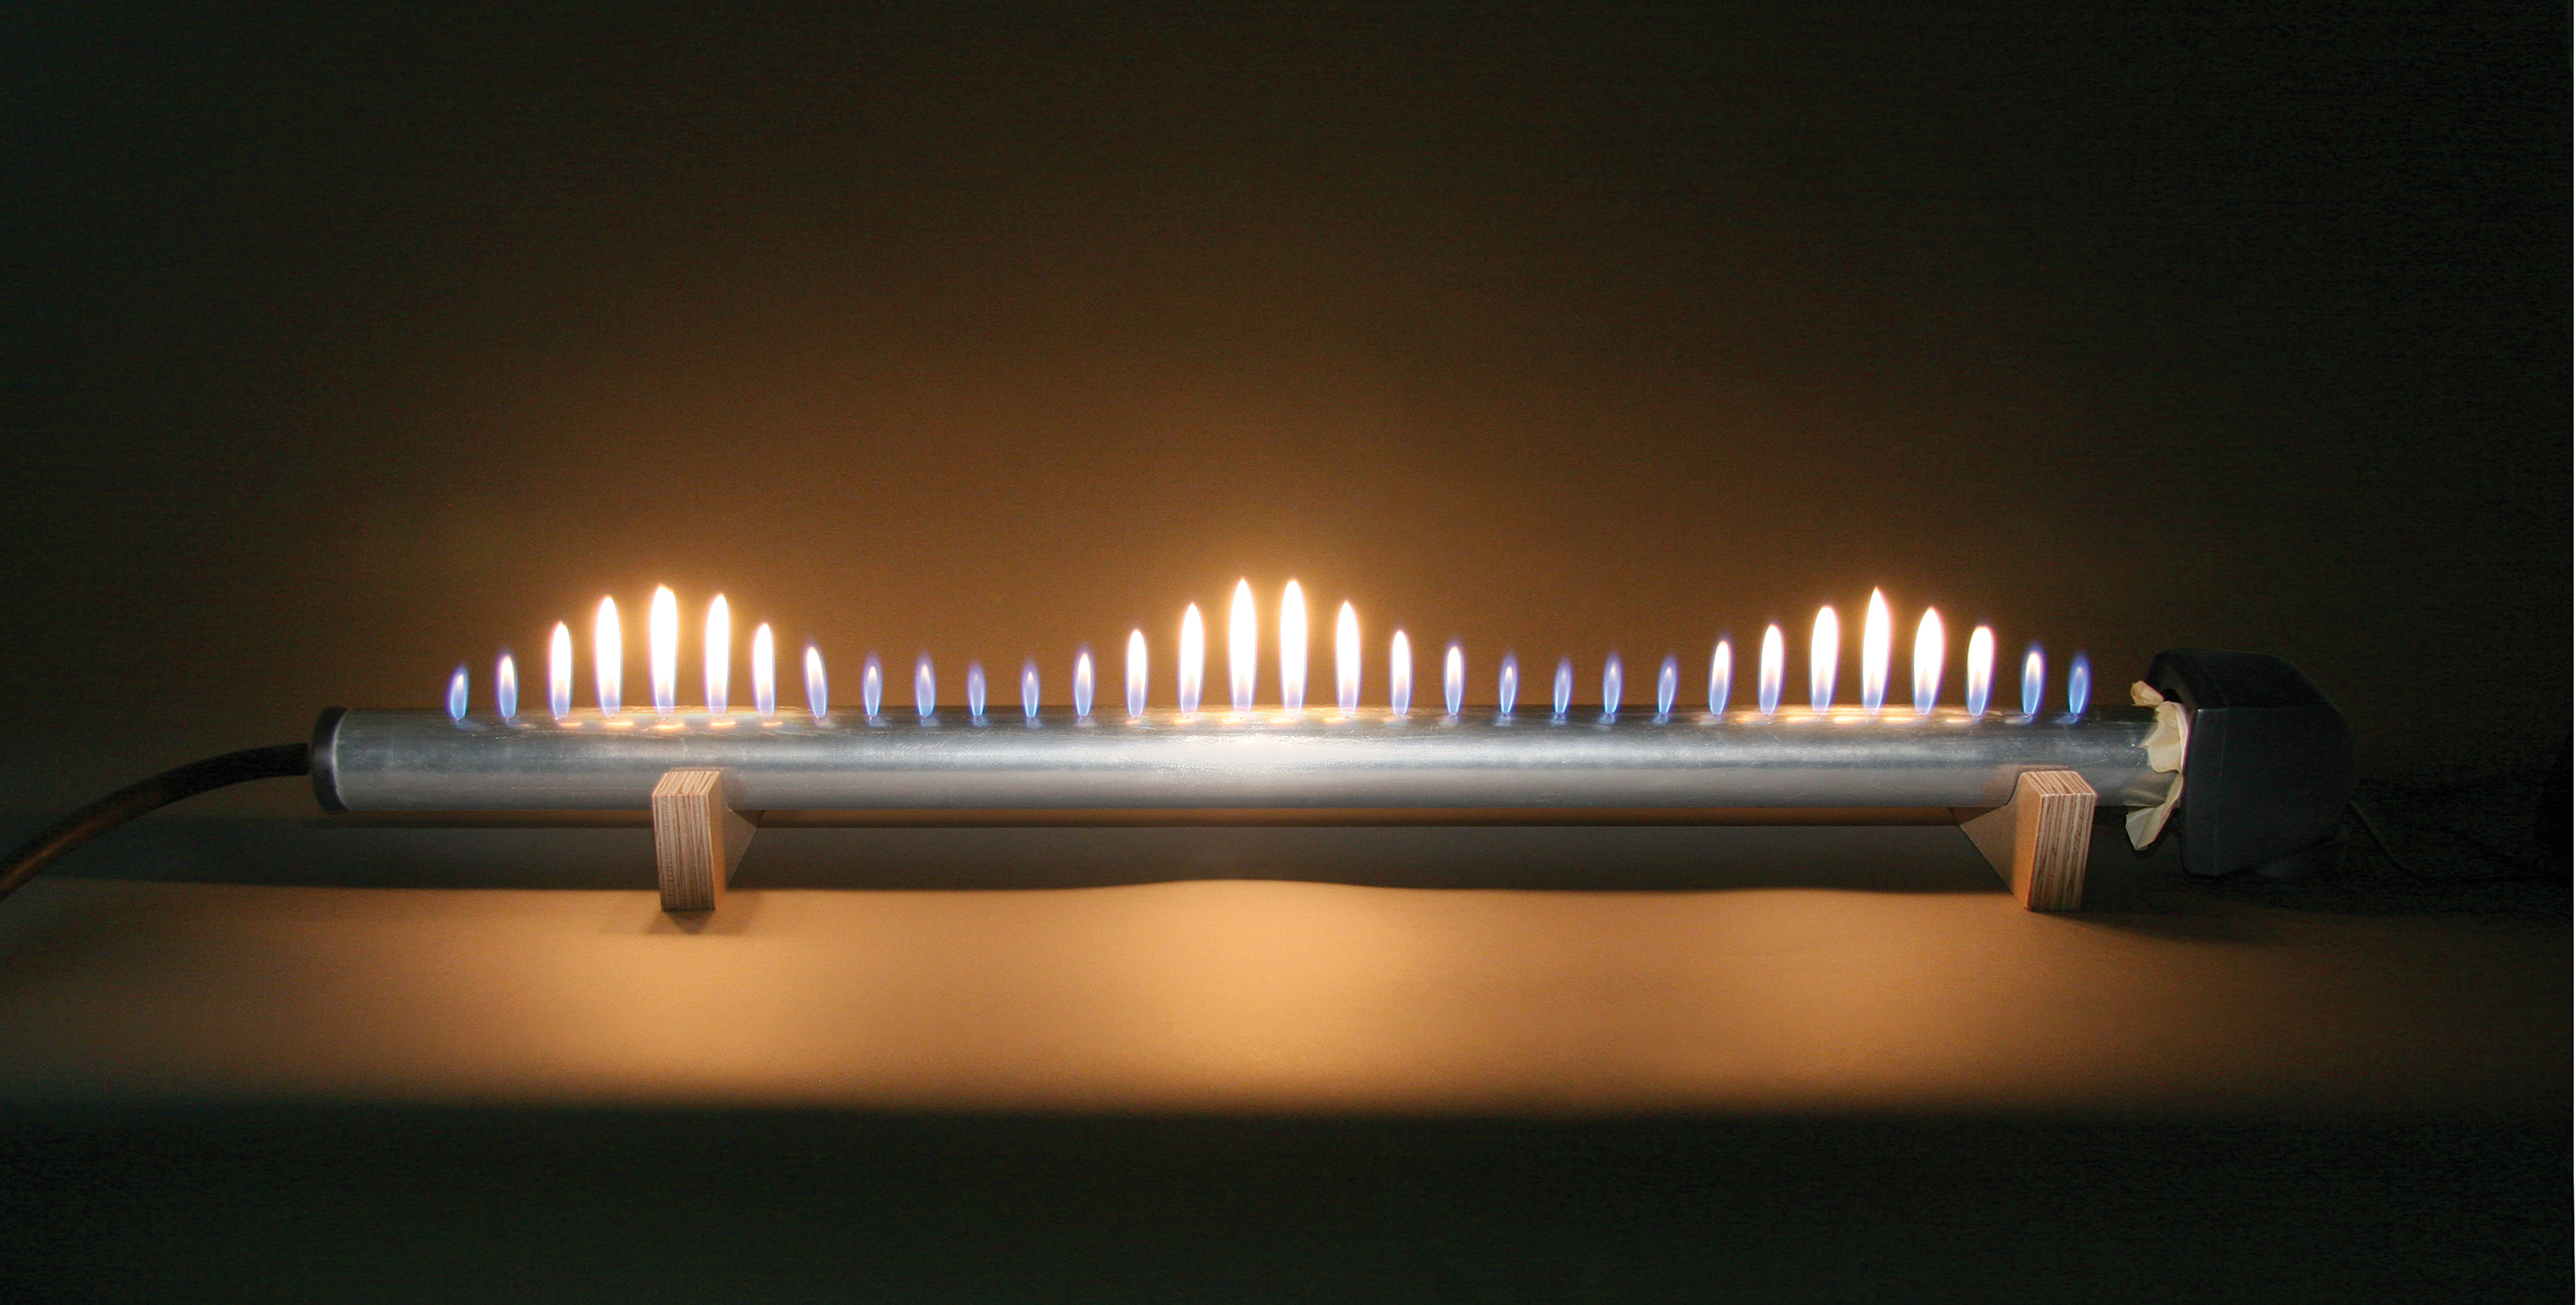
\includegraphics[scale=0.5]{images/F1.jpg}
  \caption{Imagem das chamas em um Tubo de Rubens}
\end{figure}

O comprimento do tubo é fixo, e pelo vídeo, pode ser calculado:

\begin{figure}[H]
  \centering
  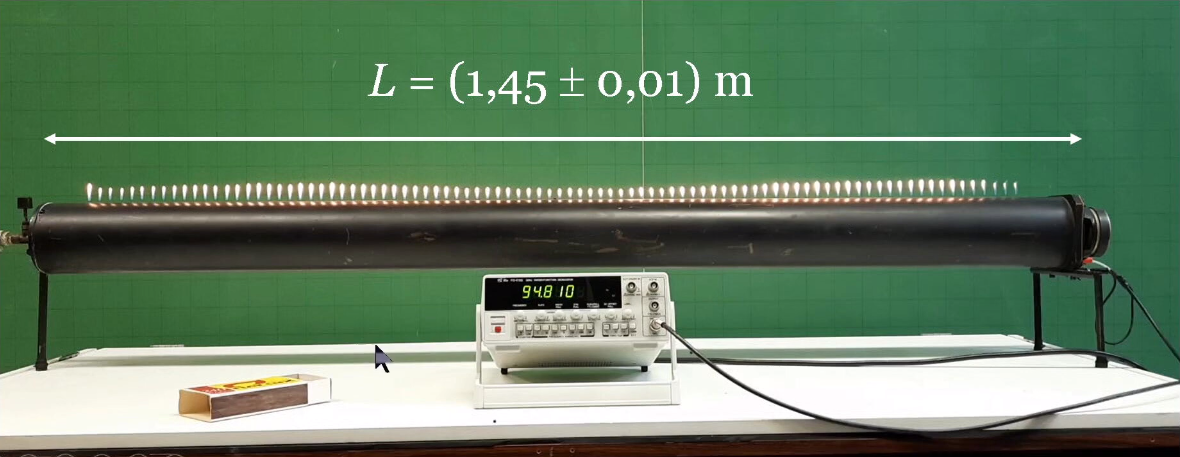
\includegraphics[scale=0.6]{images/0.png}
  \caption{Comprimento do nosso Tubo de Rubens}
\end{figure}

Analisaremos as frequências em cada um dos modos normais, notando os máximos e os nós de pressão, e montaremos uma tabela, para facilitar. Com essas informações e utilizando a fórmula a seguir, poderemos criar um gráfico da frequência $f_n$ em função de n/2L, para assim, obtermos a velocidade do som nesse gás quente - no nosso caso, será usado o GLP.

\[ f_n = \frac{n \cdot v}{2\cdot L}  \ (\ n = 1, 2, 3, 4, ...)  \]

O coeficiente angular da reta ajustada para o gráfico de $f_n$ em função de n/2L, será a velocidade do som no dado gás.\\

\textbf{OBS}: para o cálculo do coeficiente angular da reta, usaremos o método dos mínimos quadrados, utilizando um aplicativo para celular.
